\documentclass[../main.tex]{subfiles}

\addbibresource{\subfix{../references.bib}}

\begin{document}

\ifSubfilesClassLoaded{%
    \setcounter{chapter}{10}%
    \begin{refsection}
}{}

\chapter{Memory Layout dan Addressing Modes}
\label{chap:memory-layout}

\begin{subcpmk}
  \item \textbf{Sub-CPMK 5.2:} Mengimplementasikan addressing modes untuk variabel dan arrays
\end{subcpmk}

% ============================================================
% MATERI POKOK
% ============================================================
\section{Metode Pengalamatan (Addressing Modes)}

\compiler{Addressing Modes} menentukan bagaimana operan diambil dari memori atau register pada tingkat bahasa mesin. Intermediate Code Generation bertindak sebagai jembatan antara front-end yang dependen pada bahasa sumber dan back-end yang dependen pada mesin target \cite{jhu2024compilers}.

\subsection{Jenis Pengalamatan Umum}
\begin{itemize}
    \item \textbf{Register Addressing}: Operan berada langsung di register (\code{ADD R1, R2}). Sangat cepat karena tidak ada akses memori.
    \item \textbf{Immediate Addressing}: Operan adalah konstanta yang tertanam dalam instruksi (\code{ADDI R1, R1, 10}).
    \item \textbf{Displacement/Indexed}: Mengakses memori dengan alamat \textit{base register} ditambah \textit{offset} (\code{LW R1, 8(R2)}). Sangat berguna untuk \textit{stack frame} dan akses \textit{struct}.
\end{itemize}

\subsection{Complex Addressing Modes (CISC)}
Arsitektur seperti x86 mendukung mode yang lebih kompleks untuk mendukung abstraksi bahasa tingkat tinggi secara langsung di perangkat keras:
\[ \text{Alamat Efektif} = \text{Base} + (\text{Index} \times \text{Scale}) + \text{Displacement} \]
Di mana \textit{Scale} biasanya bernilai 1, 2, 4, atau 8—cocok untuk ukuran data dasar (\texttt{char}, \texttt{short}, \texttt{int}, \texttt{double}).

\subsection{Instruksi LEA (Load Effective Address)}
Instruksi \code{LEA} pada x86 adalah "trik" yang sering digunakan kompilator. Meskipun secara teknis merupakan instruksi pengalamatan, \code{LEA} sebenarnya melakukan kalkulasi aritmatika tanpa mengakses memori.
\begin{itemize}
    \item Contoh: \code{LEA EAX, [EBX + ECX*4]} menghitung $EBX + 4 \times ECX$ dan menyimpan hasilnya di EAX.
    \item Kompilator menggunakan ini untuk perkalian cepat (misal: kali 5, kali 9) dalam satu instruksi.
\end{itemize}

\begin{figure}[!htbp]
    \centering
    \adjustbox{max width=0.8\textwidth,center}{%
    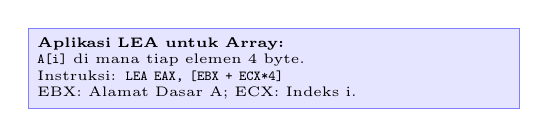
\begin{tikzpicture}[
        rect/.style={rectangle, draw=blue!50, fill=blue!10, text width=6cm, font=\tiny}
    ]
    \node[rect] (lea) {
        \textbf{Aplikasi LEA untuk Array:}\\
        \texttt{A[i]} di mana tiap elemen 4 byte.\\
        Instruksi: \texttt{LEA EAX, [EBX + ECX*4]}\\
        EBX: Alamat Dasar A; ECX: Indeks i.
    };
    \end{tikzpicture}%
    }
    \caption{Efisiensi Pengalamatan Kompleks pada Kompiler}
\end{figure}

\section{Filosofi Pengalamatan: RISC vs CISC}

Arsitektur target sangat mempengaruhi bagaimana kompilator menghasilkan kode untuk mengakses data. Dua filosofi utama adalah \compiler{CISC} (x86) dan \compiler{RISC} (RISC-V, ARM).

\subsection{CISC: Kaya dan Kompleks}
Pada x86, filosofinya adalah menyediakan instruksi yang mampu melakukan banyak hal sekaligus.
\begin{itemize}
    \item \textbf{Memory-to-Memory}: Memungkinkan operan diambil dari memori, diproses, dan hasilnya disimpan kembali ke memori dalam satu instruksi.
    \item \textbf{Variable Length}: Instruksi bisa berukuran mulai dari 1 hingga 15 byte, tergantung kompleksitas pengalamatannya.
\end{itemize}

\subsection{RISC: Sederhana dan Cepat}
Pada RISC-V atau ARM, filosofinya adalah "Load/Store Architecture".
\begin{itemize}
    \item \textbf{Terisolasi}: Hanya instruksi khusus (\code{LOAD} dan \code{STORE}) yang boleh mengakses memori. Instruksi aritmatika hanya boleh bekerja pada register.
    \item \textbf{Decomposisi}: Kompilator harus memecah akses kompleks menjadi urutan instruksi sederhana.
\end{itemize}

\subsection{Perbandingan Dekomposisi Kode}
Akses ke \code{x = a[i]} di mana \code{a} adalah array global:

\textbf{x86 (CISC)}:
\begin{lstlisting}[language={[x86masm]Assembler}]
MOV EAX, [base_a + ECX*4] ; 1 instruksi langsung
\end{lstlisting}

\textbf{RISC-V (RISC)}:
\begin{lstlisting}[language=bash]
SLLI t1, t0, 2      # t1 = i * 4 (shift left logical)
LA   t2, base_a     # Muat alamat dasar a ke t2
ADD  t3, t1, t2     # t3 = alamat elemen yang dituju
LW   a0, 0(t3)      # Muat nilai dari memori ke register
\end{lstlisting}

\begin{figure}[!htbp]
    \centering
    \adjustbox{max width=0.8\textwidth,center}{%
    \begin{tikzpicture}[
        node/.style={rectangle, draw=purple!50, fill=purple!10, text width=5cm, font=\tiny, align=center}
    ]
    \node[node] (cisc) {CISC: Instruksi Sedikit, Kompilasi Mudah, Hardware Kompleks};
    \node[node, below=0.5cm of cisc] (risc) {RISC: Instruksi Banyak, Kompilasi Berat, Hardware Sederhana};
    \end{tikzpicture}%
    }
    \caption{Trade-off antara Kompleksitas Kompiler dan Desain CPU}
\end{figure}

\section{Array Addressing}

\subsection{One-Dimensional Arrays}

Layout memory untuk 1D array:

\begin{lstlisting}[language=C]
int arr[5] = {10, 20, 30, 40, 50};

// Memory layout (each int = 4 bytes)
// arr[0] at base_address + 0*4
// arr[1] at base_address + 1*4  
// arr[2] at base_address + 2*4
// arr[3] at base_address + 3*4
// arr[4] at base_address + 4*4

// Address calculation
int address = base_address + index * sizeof(int);
\end{lstlisting}

\subsection{Multi-Dimensional Arrays}

Row-major order untuk 2D arrays:

\begin{lstlisting}[language=C]
int matrix[3][4] = {
    {1, 2, 3, 4},
    {5, 6, 7, 8},
    {9, 10, 11, 12}
};

// Address calculation: base + (row * cols + col) * sizeof(int)
int element_address = base_address + 
                     (row * 4 + col) * sizeof(int);

// matrix[1][2] = base + (1*4 + 2)*4 = base + 6*4
\end{lstlisting}

\subsection{Array Implementation}

\begin{lstlisting}[language=C]
typedef struct {
    void *base_address;
    int element_size;
    int num_dimensions;
    int *dimensions;
    int *bounds;  // lower bounds
} ArrayDescriptor;

int calculate_address(ArrayDescriptor *arr, int *indices) {
    int offset = 0;
    int stride = 1;
    
    // Calculate offset from last dimension to first
    for (int i = arr->num_dimensions - 1; i >= 0; i--) {
        offset += (indices[i] - arr->bounds[i]) * stride;
        stride *= arr->dimensions[i];
    }
    
    return (int)arr->base_address + offset * arr->element_size;
}
\end{lstlisting}

\section{Layout Struktur dan Perataan Memori}

Kompilator tidak selalu menyimpan anggota struktur secara berdampingan tanpa celah. Ada aturan perangkat keras yang memaksa data tertentu berada di alamat yang "selaras" (\textit{aligned}).

\subsection{Perataan Memori (Memory Alignment)}
Kebanyakan prosesor modern bekerja paling efisien jika data diakses pada alamat yang merupakan kelipatan dari ukuran data tersebut.
\begin{itemize}
    \item \textbf{Natural Alignment}: \texttt{int} (4 byte) harus berada di alamat yang habis dibagi 4; \texttt{double} (8 byte) di alamat yang habis dibagi 8.
    \item Jika data tidak selaras (\textit{misaligned}), CPU mungkin perlu melakukan dua kali akses memori untuk satu data, atau bahkan menyebabkan \textit{exception}.
\end{itemize}

\subsection{Padding pada Struct}
Untuk memenuhi syarat perataan, kompilator menyelipkan byte kosong yang disebut \textit{padding}.
\begin{lstlisting}[language=C]
struct Contoh {
    char a;     // 1 byte
    // Padding: 3 byte (agar 'b' mulai di offset 4)
    int b;      // 4 byte
    short c;    // 2 byte
    // Padding: 2 byte (agar total struct kelipatan 4 atau 8)
};
\end{lstlisting}

\subsection{32-bit vs 64-bit}
Ukuran pointer dan tipe data dasar dapat berubah antar arsitektur:
\begin{itemize}
    \item \textbf{Pointer}: 4 byte pada sistem 32-bit, 8 byte pada sistem 64-bit.
    \item \textbf{Alignment Requirement}: Sistem 64-bit seringkali lebih ketat, mengharuskan lebih banyak padding untuk tipe data \texttt{long} atau pointer.
\end{itemize}

\subsection{Packed Structures}
Kompilator menyediakan direktif (seperti \texttt{\#pragma pack(1)}) untuk menghilangkan padding. Ini berguna untuk protokol jaringan atau format file, namun berisiko menurunkan performa akses memori.

\begin{figure}[!htbp]
    \centering
    \adjustbox{max width=0.8\textwidth,center}{%
    \begin{tikzpicture}[
        byte/.style={rectangle, draw, minimum width=0.5cm, minimum height=0.5cm, font=\tiny}
    ]
    \node[byte, fill=blue!20] (b1) {A};
    \node[byte, right=0pt of b1, fill=gray!20] (p1) {P};
    \node[byte, right=0pt of p1, fill=gray!20] (p2) {P};
    \node[byte, right=0pt of p2, fill=gray!20] (p3) {P};
    \node[byte, right=0pt of p3, fill=green!20, minimum width=2cm] (i1) {Integer B};
    \end{tikzpicture}%
    }
    \caption{Visualisasi Padding (P) untuk Menyelaraskan Integer B}
\end{figure}

\section{Pointer Arithmetic}

\subsection{Pointer Operations}

\begin{lstlisting}[language=C]
int arr[10] = {0, 1, 2, 3, 4, 5, 6, 7, 8, 9};
int *ptr = arr;

// Pointer arithmetic
ptr++;        // ptr += sizeof(int) (moves to next element)
ptr += 3;     // ptr += 3 * sizeof(int)
ptr--;        // ptr -= sizeof(int)

// Array access via pointers
int value = *(ptr + 2);  // Same as ptr[2]
int diff = ptr - arr;    // Number of elements between pointers
\end{lstlisting}

\subsection{Dynamic Arrays}

\begin{lstlisting}[language=C]
typedef struct {
    int *data;
    int size;
    int capacity;
} DynamicArray;

DynamicArray* create_array(int initial_capacity) {
    DynamicArray *arr = malloc(sizeof(DynamicArray));
    arr->data = malloc(initial_capacity * sizeof(int));
    arr->size = 0;
    arr->capacity = initial_capacity;
    return arr;
}

void resize_array(DynamicArray *arr, int new_capacity) {
    arr->data = realloc(arr->data, new_capacity * sizeof(int));
    arr->capacity = new_capacity;
}
\end{lstlisting}

\section{Translasi Alamat dan Performa}

Pada sistem operasi modern, alamat yang dihasilkan oleh kompilator adalah alamat logis atau \textit{virtual}. Perangkat keras (\textit{MMU}) harus memetakan ini ke alamat fisik di RAM.

\subsection{Virtual to Physical Address}
Proses translasi ini biasanya melibatkan pembagian alamat menjadi \textit{Page Number} dan \textit{Offset}. Kompilator harus memastikan data yang sering diakses bersama-sama berada dalam satu \textit{page} (halaman) yang sama untuk meminimalkan \textit{page fault}.

\subsection{TLB (Translation Lookaside Buffer)}
\textit{TLB} adalah cache khusus di dalam CPU yang menyimpan pemetaan alamat virtual ke fisik yang baru saja digunakan. 
\begin{itemize}
    \item \textbf{TLB Hit}: Alamat fisik ditemukan di TLB, akses sangat cepat.
    \item \textbf{TLB Miss}: CPU harus mencari di tabel halaman (\textit{page table}) di RAM, yang jauh lebih lambat.
\end{itemize}

\subsection{Pentingnya Lokalitas Spasial}
Manajemen memori oleh kompilator (seperti pemilihan \textit{Row-Major order}) sangat krusial karena mendukung \textbf{Lokalitas Spasial}.
\begin{itemize}
    \item Jika elemen array diakses secara berurutan sesuai layout memori, maka data tersebut kemungkinan besar sudah ada di cache CPU dan pemetaan halamannya sudah ada di TLB.
    \item Lompatan alamat yang acak atau besar dapat menyebabkan \textit{TLB Miss} dan \textit{Cache Miss} berulang kali, menurunkan performa program secara drastis meskipun algoritma di tingkat tinggi tampak efisien.
\end{itemize}

\begin{figure}[!htbp]
    \centering
    \adjustbox{max width=0.8\textwidth,center}{%
    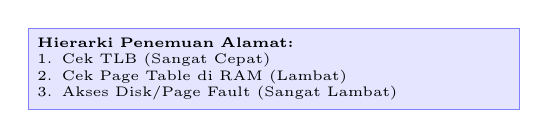
\begin{tikzpicture}[
        seg/.style={rectangle, draw=blue!50, fill=blue!10, text width=6cm, font=\tiny}
    ]
    \node[seg] (tlb) {
        \textbf{Hierarki Penemuan Alamat:}\\
        1. Cek TLB (Sangat Cepat)\\
        2. Cek Page Table di RAM (Lambat)\\
        3. Akses Disk/Page Fault (Sangat Lambat)
    };
    \end{tikzpicture}%
    }
    \caption{Alur Penemuan Alamat Fisik di Perangkat Keras}
\end{figure}


% ============================================================
% AKTIVITAS PEMBELAJARAN
% ============================================================
\begin{aktivitas}
  \item \textbf{Memory Layout}: Implementasikan simulator memory layout untuk berbagai tipe data.
  \item \textbf{Array Addressing}: Bangun array descriptor untuk multi-dimensional arrays.
  \item \textbf{Pointer Arithmetic}: Implementasikan pointer arithmetic operations.
  \item \textbf{Structure Layout}: Analisis memory layout untuk structures dengan padding.
  \item \textbf{Address Translation}: Implementasikan simple virtual memory translation.
\end{aktivitas}

% ============================================================
% LATIHAN DAN REFLEKSI
% ============================================================
\begin{latihan}
  \item Hitung memory layout untuk struktur dengan nested structures!
  \item Implementasikan address calculation untuk 3D array dengan arbitrary bounds!
  \item Analisis overhead dari different addressing modes!
  \item Desain memory layout untuk object-oriented language dengan inheritance!
  \item Implementasikan garbage collection-aware memory management!
  \item \textbf{Refleksi}: Bagaimana memory layout mempengaruhi performance program?
\end{latihan}

% ============================================================
% ASESMEN
% ============================================================
\begin{asesmen}
\textbf{Instrumen Penilaian untuk Sub-CPMK 5.2}

\textbf{A. Pilihan Ganda}

\begin{enumerate}
  \item Row-major order untuk 2D array menghitung:
  \begin{enumerate}
    \item row * cols + col
    \item col * rows + row
    \item row + col * cols
    \item col + row * rows
  \end{enumerate}
  
  \item Structure padding digunakan untuk:
  \begin{enumerate}
    \item Mengurangi memory usage
    \item Alignment optimization
    \item Error detection
    \item Security
  \end{enumerate}
  
  \item Pointer arithmetic pada int pointer menambah:
  \begin{enumerate}
    \item 1 byte
    \item 2 bytes
    \item 4 bytes
    \item 8 bytes
  \end{enumerate}
\end{enumerate}

\textbf{B. Essay}

\begin{enumerate}
  \item Jelaskan implementasi complete addressing modes untuk bahasa dengan arrays, structures, dan pointers!
  \item Desain memory layout system yang efisien untuk dynamic data structures!
\end{enumerate}

\textbf{Rubrik Penilaian}: Lihat Lampiran A
\end{asesmen}

% ============================================================
% CHECKLIST KOMPETENSI
% ============================================================
\begin{checklist}
  \item Saya dapat mengimplementasikan addressing modes untuk variabel dan arrays
  \item Saya dapat menghitung memory layout untuk structures dan unions
  \item Saya dapat melakukan pointer arithmetic operations
  \item Saya dapat mengimplementasikan array descriptor systems
  \item Saya memahami virtual memory address translation
  \item Saya dapat mendesain efficient memory layouts
\end{checklist}

% ============================================================
% RANGKUMAN
% ============================================================
\begin{rangkuman}
Bab ini membahas memory layout dan addressing modes, termasuk storage classes, addressing modes, array implementation, structure layout, pointer arithmetic, dan address translation. Mahasiswa belajar mengimplementasikan efficient memory management.

\textbf{Poin Kunci:}
\begin{itemize}
  \item Memory layout menentukan bagaimana data disimpan dan diakses
  \item Addressing modes menyediakan berbagai cara mengakses data
  \item Array addressing memerlukan perhitungan offset yang tepat
  \item Structure layout mempertimbangkan alignment dan padding
  \item Pointer arithmetic memungkinkan efficient data access
  \item Virtual memory translation memisahkan logical dan physical addresses
\end{itemize}

\textbf{Kata Kunci}: \compiler{Memory Layout}, \compiler{Addressing Modes}, \compiler{Array Addressing}, \compiler{Structure Layout}, \compiler{Pointer Arithmetic}, \compiler{Virtual Memory}, \compiler{Memory Alignment}
\end{rangkuman}

\ifSubfilesClassLoaded{%
    \clearpage
    \printbibliography[title={Daftar Pustaka}]
    \end{refsection}
}{}

\end{document}
